For all parts of this question I have assumed $T = 300 \textrm{ K}$ and have used values appropriate for silicon.
\subsection*{a)}
	\begin{figure}[htbp!]
		%	\centering
		\flushright
		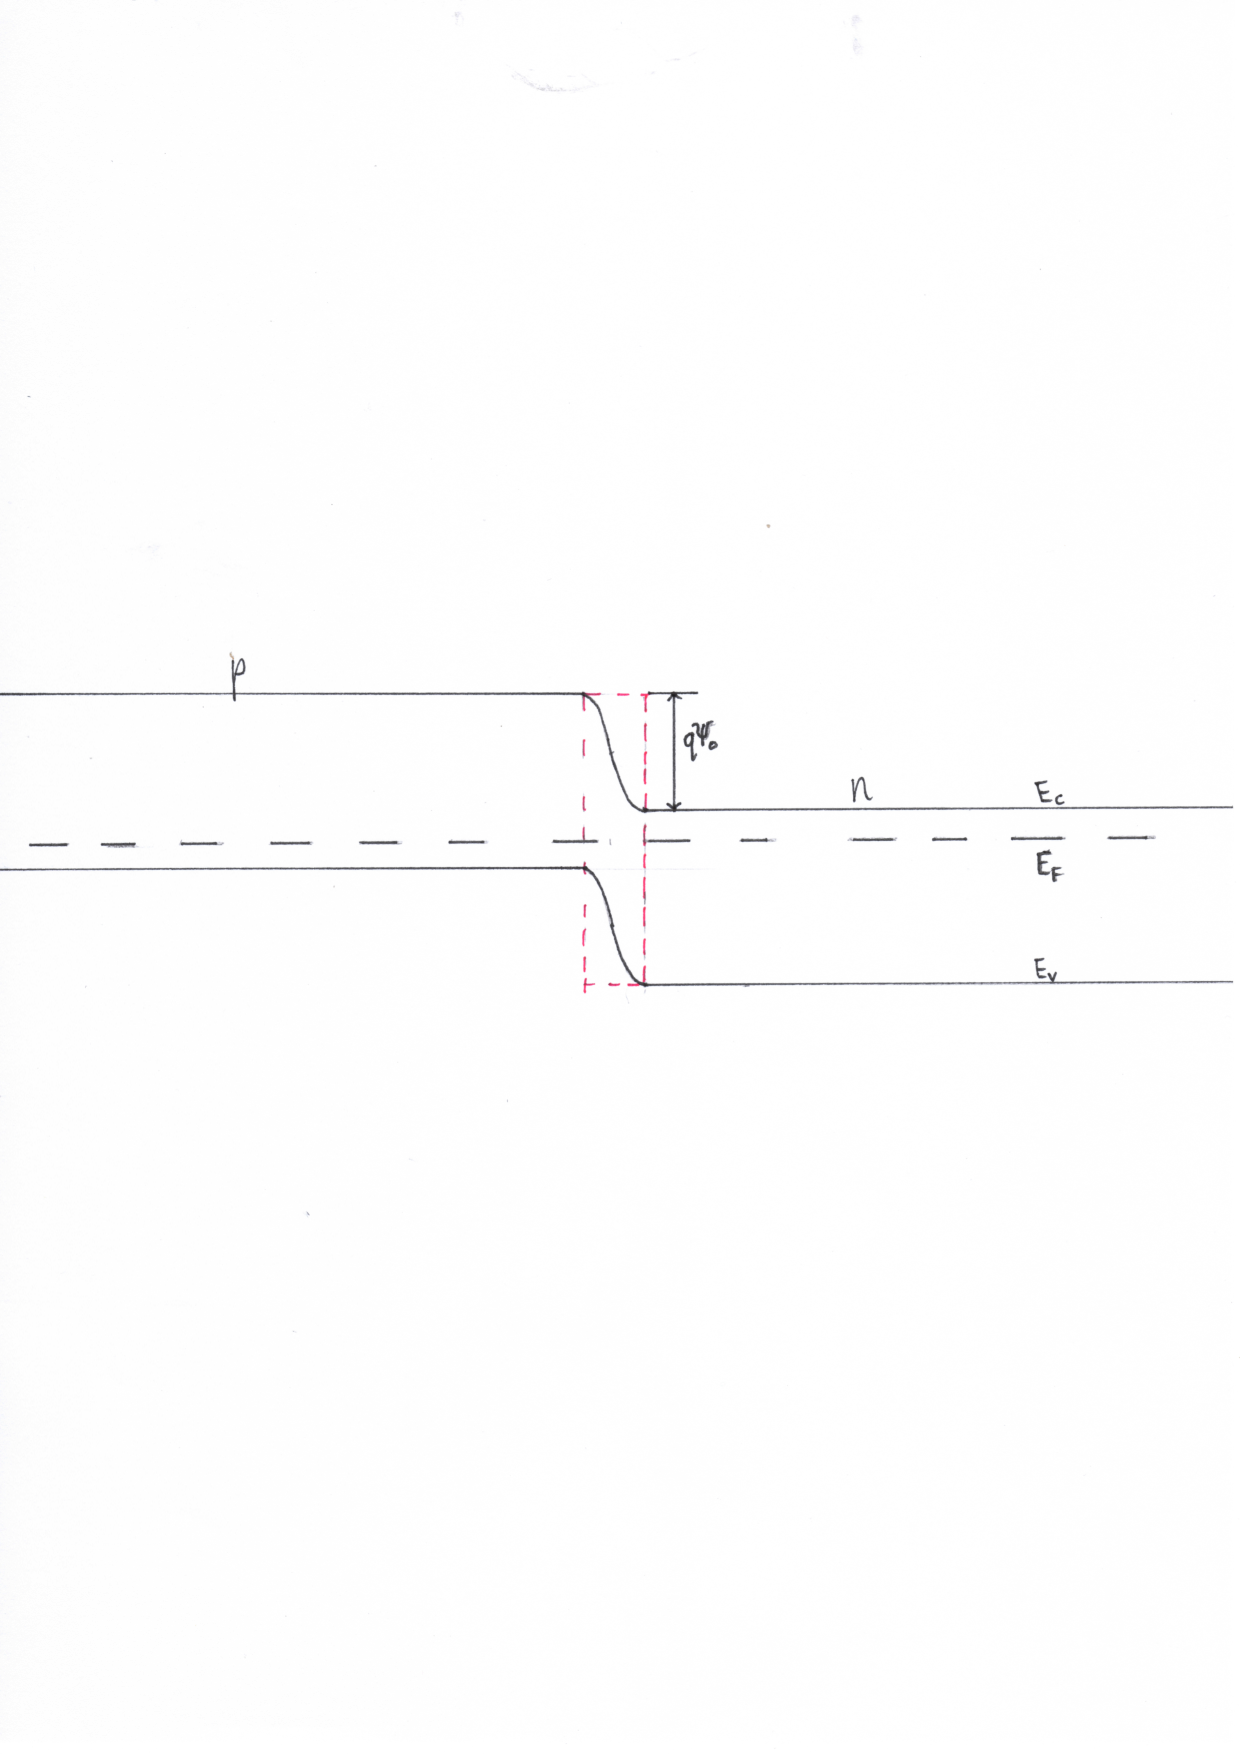
\includegraphics[trim={3.5cm 12.5cm 2.5cm 11cm},clip]{./img/2a}
		\caption{Energy diagram of a pn junction.}
	\end{figure}
	\[
	\begin{aligned}
		q \psi_0 &= E_C(p) - E_C(n) \\
			   &= (E_F + E_G - E_1) - (E_F + E_2) \\
			   &= E_G - E_1 - E_2 \\
			   &= 1.12 \textrm{ eV} - k T \ln \left( \frac{N_V N_C}{N_A N_D} \right) \\
			\psi_0  &=	1.12 \textrm{ V} - 0.147 \textrm{ V} \\
			   &= 0.973 \textrm{ V}	   
	\end{aligned}
	\]
\subsection*{b)}
	Under forward-bias, electrons are injected into the n-doped regions, and positive charges, or holes, 
	will be injected into the p-doped region. An electron injected into the n-doped region will feel an electric attraction due to the positive-space charge region and so will accelerate, and be swept into the p-doped region, as a drift current. Once in the p-region, it can readily recombine with a hole. Once carriers have recombined, we have reached our initial conditions, and the process will repeat. Due to the recombination current, more current will be drawn from the applied voltage source. A similar explanation can be applied to the holes injected into the p-doped region, being swept into the n-doped region. Therefore, the minority carriers define the large portion of the total diode current.
\subsection*{c)}
	Poisson's equation can be expressed as
	$$-\dfrac{d^2 V}{d x^2} = \dfrac{d\hat{E}}{dx} = \frac{\rho}{\epsilon} %= \frac{q}{\epsilon}(p - n + N^{+}_D - N^{-}_A)
	$$
	
	If we assume the depletion approximation, the electric field will be confined to the transition region of the pn junction. $\rho$ is the charge carrier density, and is assumed to be constant throughout the p doped region, with a value of $q N_A$, and also throughout the n doped region as $q N_D$.
	
	Therefore, for $x_p \le x < 0$, we can solve
	\[
	\begin{aligned}
		\dfrac{d\hat{E}}{dx} &= -\frac{q N_A}{\epsilon} \\
					\hat{E}	 &= -\frac{q N_A}{\epsilon} x + c
	\end{aligned}
	\]
	Applying the depletion approximation, and asserting a continuity in electric field $\hat{E}$, we know that $\hat{E} = 0$ when $x = x_p$, noting that $x_p < 0$.
	\[
	\begin{aligned}
		\therefore c &= - \dfrac{q N_A}{\epsilon}\left|x_p\right| \\
		\therefore \hat{E}(x) &= - \dfrac{q N_A}{\epsilon}(\left|x_p\right| + x) \textrm{\hspace{0.5cm} for } x_p \le x < 0
	\end{aligned}
	\]
	Similarly, for the n-doped region,
	$$ \hat{E}(x) = \dfrac{q N_D}{\epsilon}(x -x_n) \textrm{\hspace{0.5cm} for } 0 \le x \le x_n$$
	\begin{figure}[htbp!]
		\centering
		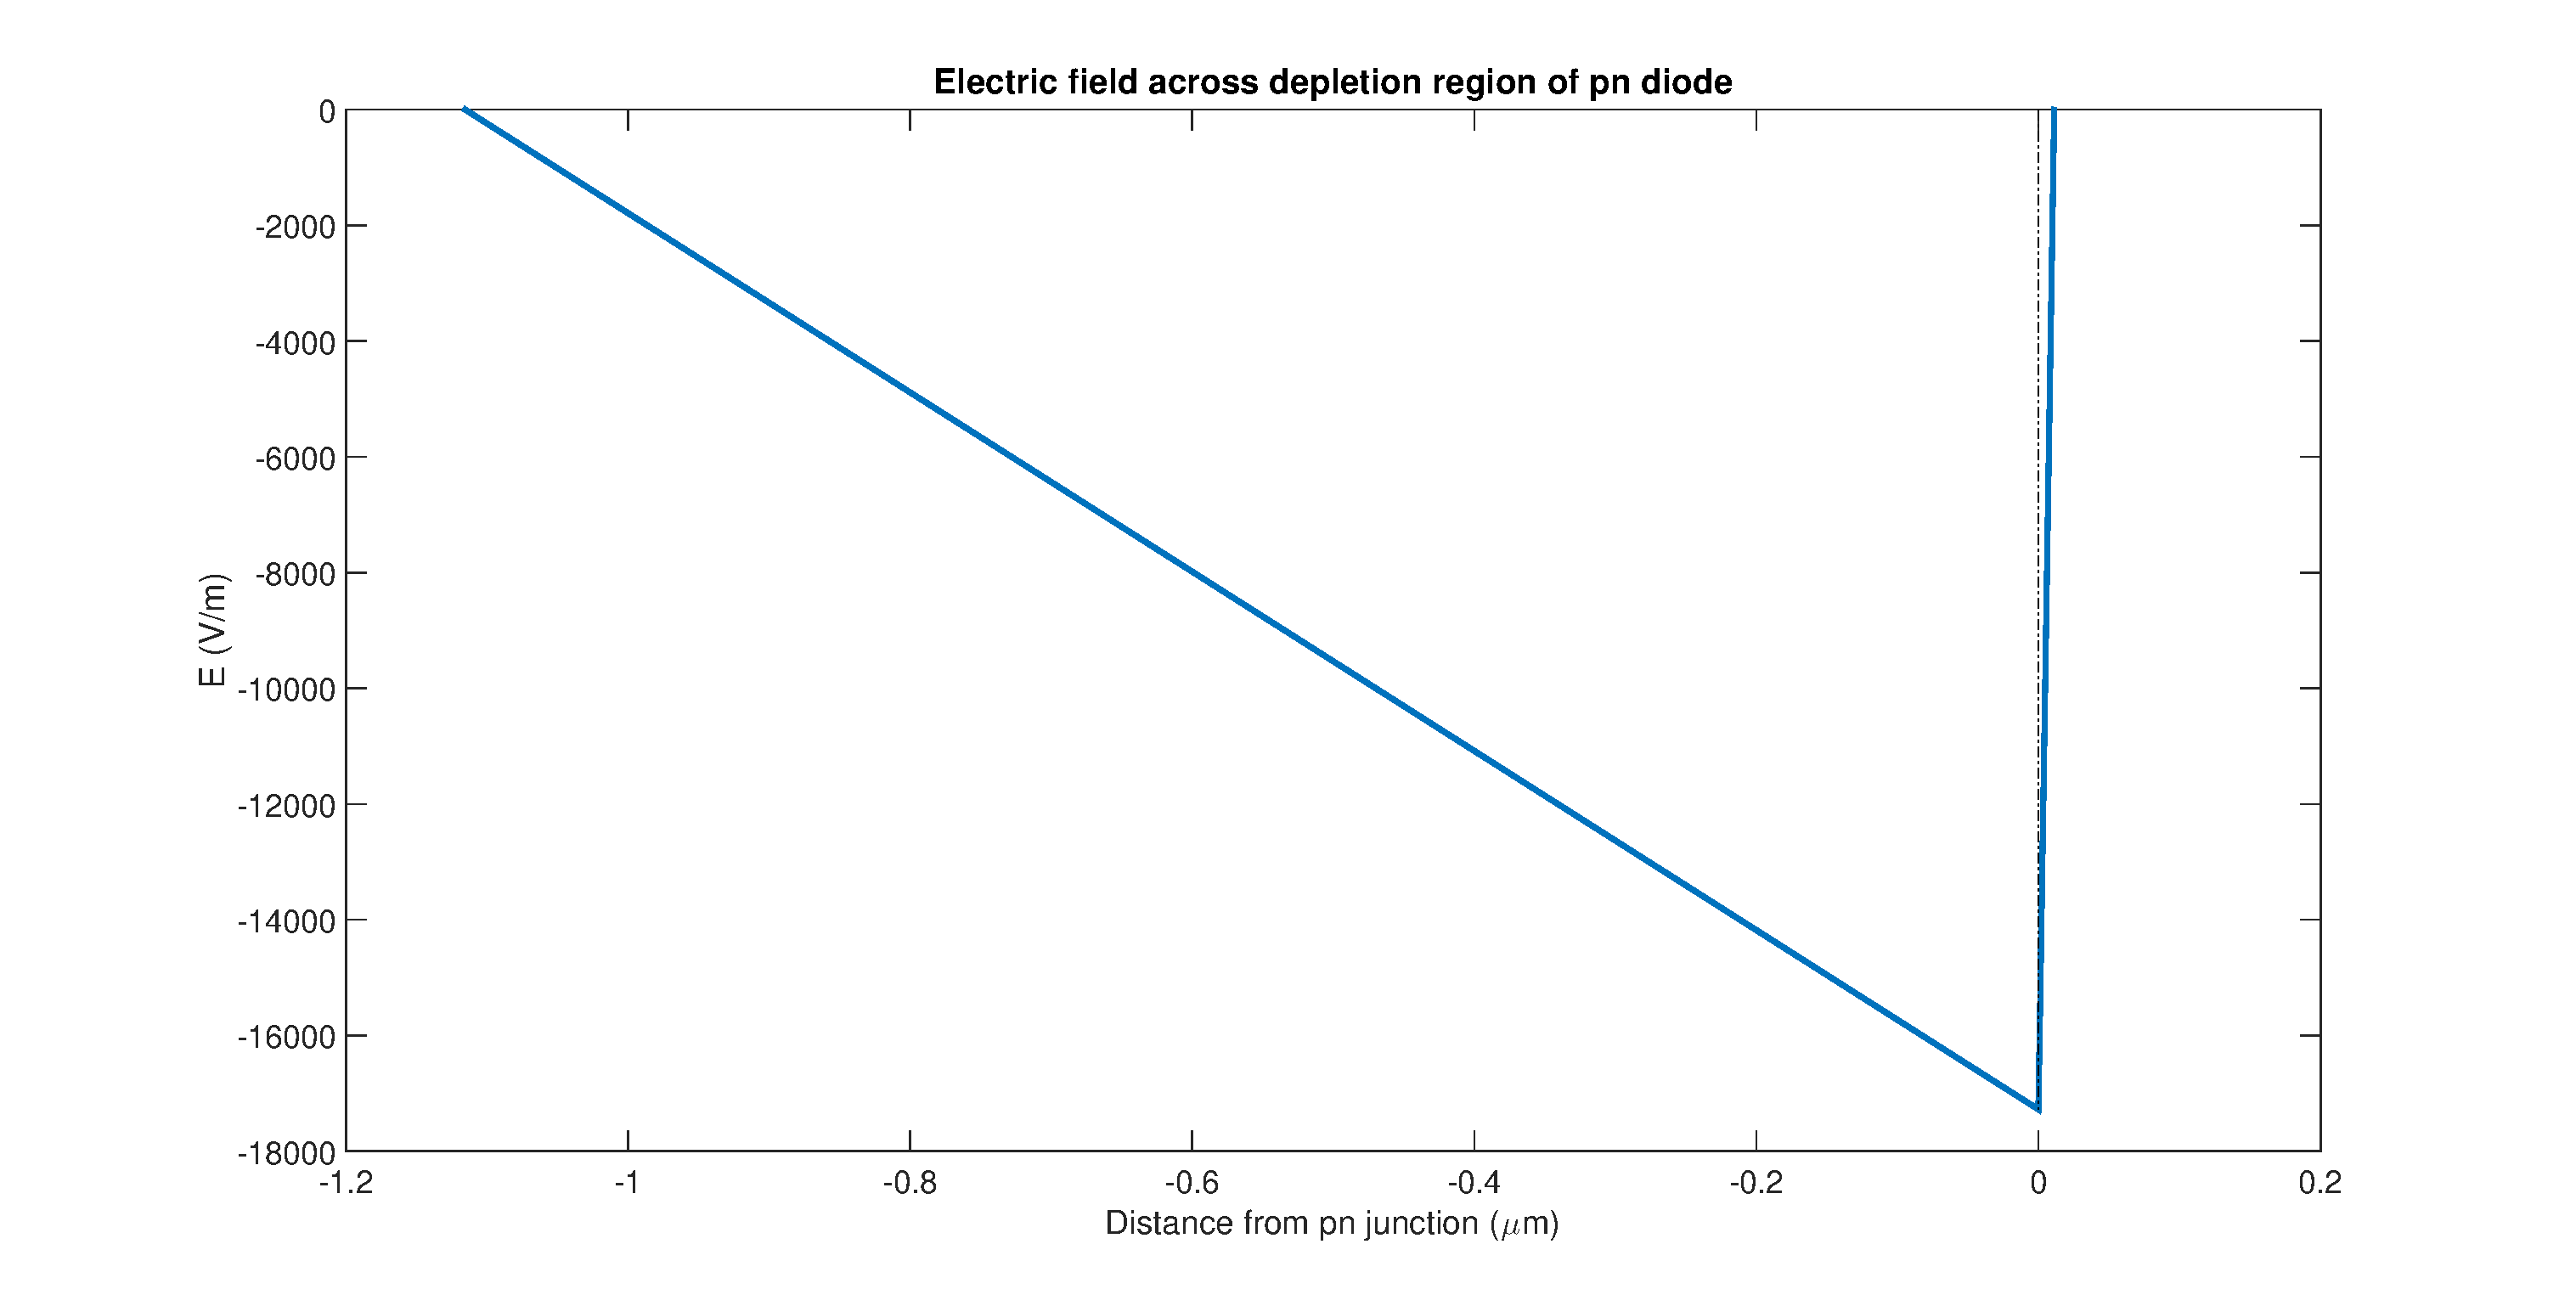
\includegraphics[width=0.8\textwidth]{./img/2c_E}
		\caption{The electric field $\hat{E}$ across the depletion region of a PN diode.}
		\label{fig::e_field}
	\end{figure}	
	A plot of this function is shown in Figure \ref{fig::e_field}.
	
	If we integrate again, we can find the built-in potential $\psi_0$.
	\[
	\begin{aligned}
		- \dfrac{d \psi_0}{dx} &= \hat{E} \\
		\psi_0 &= - \int_{x_p}^{x_n} \hat{E} dx \\
			   &= 
			   \int_{x_p}^{0} \frac{q N_A}{\epsilon} (\left|x_p\right|+x) dx 
			   - \int_{0}^{x_n} \frac{q N_D}{\epsilon} (x - x_n) dx \\
			   &= \dfrac{q N_A}{2 \epsilon} x_p^2 + \dfrac{q N_D}{2 \epsilon} x_n^2 \\
			   &= 0.973 \textrm{ V}
	\end{aligned}
	\]
	
	A plot of the built-in potential as a function of space is shown in Figure \ref{fig::built_in}.
	
	\begin{figure}[htbp!]
		\centering
		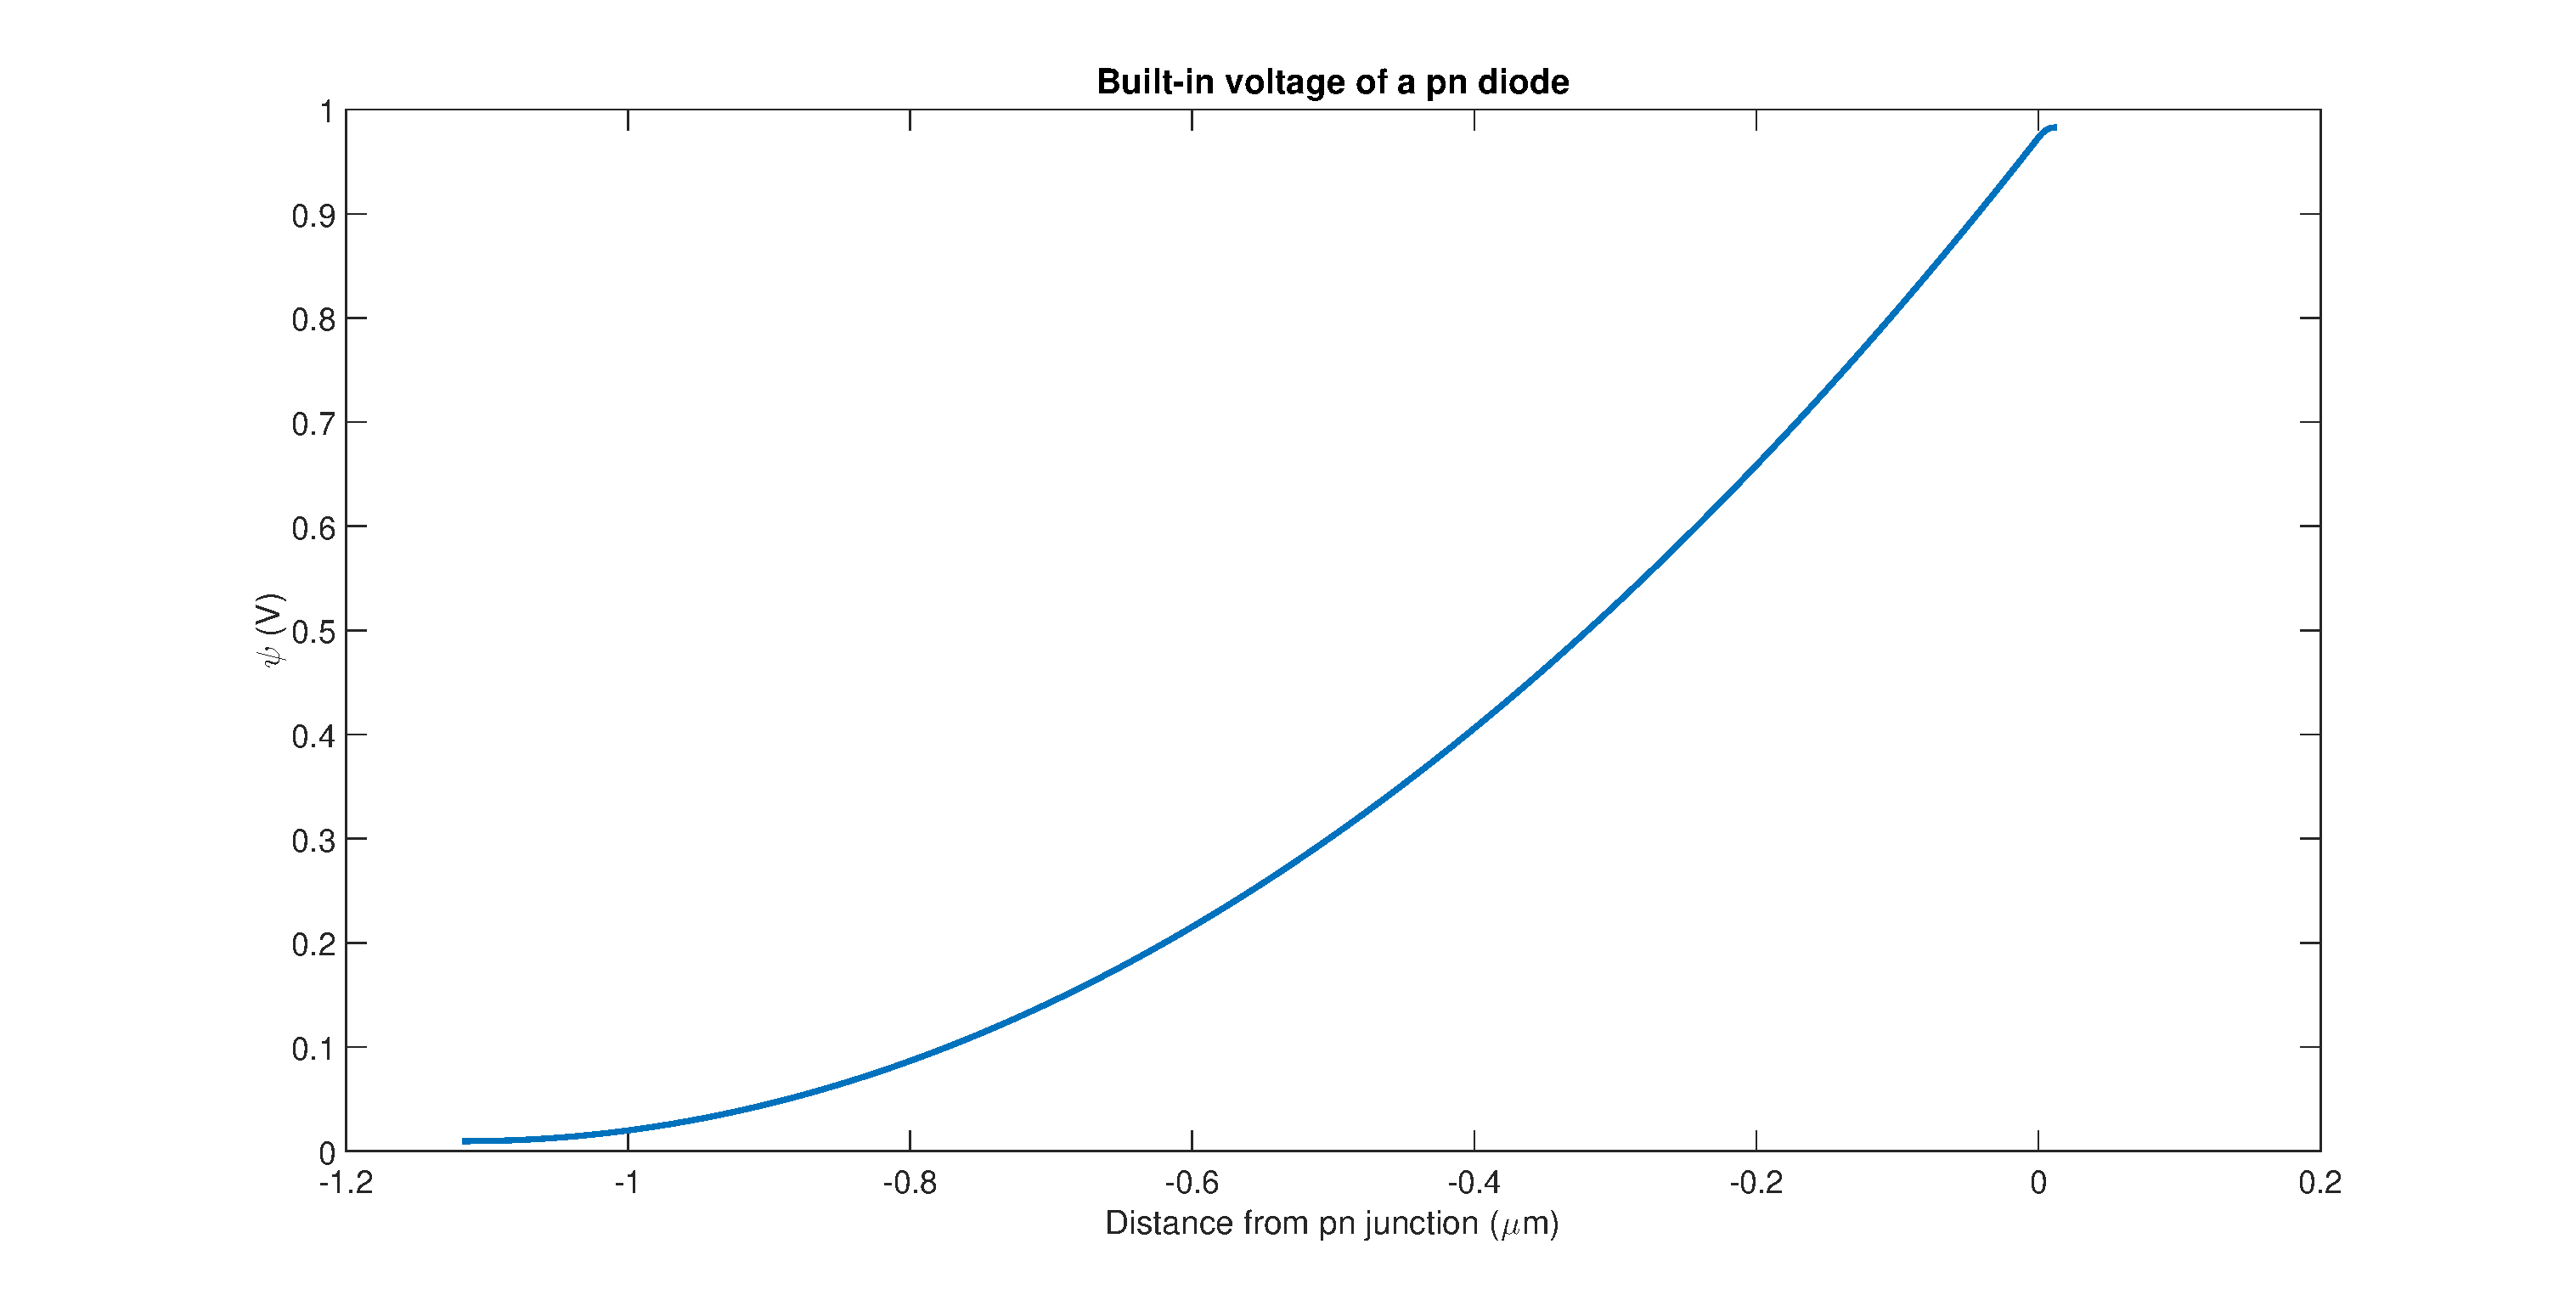
\includegraphics[width=0.8\textwidth]{./img/2c_psi}
		\caption{The built-in voltage $\psi$ across the depletion region of a PN diode.}
		\label{fig::built_in}
	\end{figure}
